\documentclass[sigplan,10pt,anonymous,review]{acmart}\settopmatter{printfolios=true,printccs=false,printacmref=false}


\usepackage[utf8]{inputenc}
\usepackage{microtype} % Better typesetting for PDFs -- is enabling this ok?
\usepackage{balance}

\usepackage{amsmath}
\usepackage{amssymb}
\usepackage{amsthm}

%\usepackage{eufrak} %The eufrak package is redundant if the amsfonts package is used
\usepackage{mathpartir}
\DeclareMathAlphabet{\mathpzc}{OT1}{pzc}{m}{it}
\usepackage[boxed]{algorithm}
\usepackage{enumerate}
\usepackage{cprotect}

\usepackage{listings}
\usepackage{lstautogobble}
\usepackage{graphicx}
\usepackage{tabularx}
\usepackage{booktabs}
\usepackage{ragged2e}  % for '\RaggedRight' macro (allows hyphenation)
\usepackage{color}
\usepackage[noend]{algpseudocode}
\usepackage{caption}
\usepackage[font=scriptsize]{subcaption}
\usepackage{hyperref}
\usepackage{float}
\usepackage{wrapfig}

\usepackage{multirow}
\usepackage{siunitx}

\usepackage{tikz}
\usetikzlibrary{positioning,fit,shadows,decorations, arrows, shapes, decorations.markings,decorations.pathmorphing,calc}

\tikzset{
  -|-/.style={
    to path={
      (\tikztostart) -| ($(\tikztostart)!#1!(\tikztotarget)$) |- (\tikztotarget)
      \tikztonodes
    }
  },
  -|-/.default=0.5,
  |-|/.style={
    to path={
      (\tikztostart) |- ($(\tikztostart)!#1!(\tikztotarget)$) -| (\tikztotarget)
      \tikztonodes
    }
  },
  |-|/.default=0.5,
}

\clubpenalty = 10000
\widowpenalty = 10000
\displaywidowpenalty = 10000

% Not really meant for highlighting isabelle source, but for easily writing latex that looks like
% isabelle
% 
% keyword level 1 - isabelle outer syntax 
% keyword level 2 - isabelle inner syntax programming constructs (if, let, etc)
% keyword level 3 - standard constants (length, mod, etc)
% keyword level 4 - isabelle proof methods


% \newcommand{\lsem}{\ensuremath{\mathopen{[\![}}}
% \newcommand{\rsem}{\ensuremath{\mathclose{]\!]}}}

\lstdefinelanguage{isabelle}{
  morekeywords={theorem,theorems,corollary,lemma,lemmas,locale,begin,end,fixes,assumes,shows,and,class,
    constrains , definition, where, apply, done,unfolding, primrec, fun, using, by, for, uses, file,
    schematic_lemma, concrete_definition, prepare_code_thms, export_code, datatype, type_synonym, typedef, value,
    proof, next, qed, show, have, hence, thus, interpretation, fix, context, sepref_definition,is,export_llvm
 } ,
  morekeywords=[2]{rec, return, bind, foreach, if, then, else, do, let, in, res, spec, fail, assert, while, case, of, 
    check},
%  morekeywords=[3]{length,mod,insert},
%   morekeywords=[4]{simp,auto,intro,elim,rprems,refine_mono,refine_rcg},
  sensitive=True,
  morecomment=[s]{(\*}{\*)},
}


\DeclareTextCommand{\shortunderscore}{T1}{{$\lambda$}}1
  {\\\%}{{$\lambda$}}1
  {\\\$}{{$\mathbin{\,\$\,}$}}1
  {->}{{$\rightarrow$}}1
  {<-}{{$\leftarrow$}}1
  {<.}{{$\langle$}}1
  {.>}{{$\rangle$}}1
  {<=}{{$\le$}}1
  {>=}{{$\ge$}}1
  {<->}{{$\leftrightarrow$}}1
  {-->}{{$\longrightarrow$}}2
  {<-->}{{$\longleftrightarrow$}}1
  {=>}{{$\Rightarrow$}}1
  {==}{{$\equiv$}}2
  {==>}{{$\implies$}}2
  {<=>}{{$\Leftrightarrow$}}1
  {~=}{{$\ne$}}1
  {|}{{$\mid$}}1
  {-`}{{$\rightharpoonup$}}1
  {|`}{{$\restriction$}}1
  {!!}{{$\bigwedge$}}1
  {(}{{$($}}1
  {)}{{$)$}}1
  {\{}{{$\{$}}1
  {\}}{{$\}$}}1
  {[}{{$[$}}1
  {]}{{$]$}}1
  {[|}{{$\llbracket$}}1
  {|]}{{$\rrbracket$}}1
  {\\<lbrakk>}{{$\lsem$}}1
  {\\<rbrakk>}{{$\rsem$}}1
  {|-}{{$\vdash$}}1
  {|=}{{$\models$}}1
  {|->}{{$\mapsto$}}1
  {|_|}{{$\bigsqcup$}}1
  {...}{{$\dots$}}1
  {\\x}{{$\times$}}1
  {_0}{{${}_0$}}1
  {_1}{{${}_1$}}1
  {_2}{{${}_2$}}1
  {_3}{{${}_3$}}1
  {_4}{{${}_4$}}1
  {_5}{{${}_5$}}1
  {_6}{{${}_6$}}1
  {_7}{{${}_7$}}1
  {_8}{{${}_8$}}1
  {_9}{{${}_9$}}1
  {_L}{{${}_L$}}1
  {\\_n}{{${}_n$}}1
  {\\_i}{{${}_i$}}1
  {\\_j}{{${}_j$}}1
  {\\_x}{{${}_x$}}1
  {\\_y}{{${}_y$}}1
  {\\impl}{{${}_\dagger$}}1
  {^*}{{$^*$}}1
  {^k}{{$^k$}}1
  {^d}{{$^d$}}1
  {\\<^sup>*}{{$^*$}}1
  {\\<^sub>*}{{$_*$}}1
  {\\<^sub>A}{{$_A$}}1
  {\\<^sub>r}{{$_r$}}1
  {\\<^sub>a}{{$_a$}}1
  {:_i}{{$:_i$}}1
  {\\<A>}{{$\mathcal{A}$}}1
  {\\<O>}{{\sf o}}1
  {\\<Phi>}{{$\Phi$}}1
  {\\<Psi>}{{$\Psi$}}1
  {\\<sigma>}{{$\sigma$}}1
  {\\<cdot>}{{$\cdot$}}1
  {\\<in>}{{$\in$}}1
  {\\<le>}{{$\le$}}1
  {\\<noteq>}{{$\ne$}}1
  {\\<lambda>}{{$\lambda$}}1
  {\\<longrightarrow>}{{$\longrightarrow$}}1
  {\\<longleftrightarrow>}{{$\longleftrightarrow$}}1
  {\\<Rightarrow>}{{$\Rightarrow$}}1
  {\\<Longrightarrow>}{{$\Longrightarrow$}}1
  {\\<rightarrow>}{{$\rightarrow$}}1
  {\\<leftarrow>}{{$\leftarrow$}}1
  {\\<mapsto>}{{$\mapsto$}}1
  {\\<equiv>}{{$\equiv$}}1
  {\\<and>}{{$\wedge$}}1
  {\\<or>}{{$\vee$}}1
  {\\<And>}{{$\bigwedge$}}1
  {\\<Up>}{{$\Uparrow$}}1
  {\\<Down>}{{$\Downarrow$}}1
  {\\<Union>}{{$\bigcup$}}1
  {\\<up>}{{$\uparrow$}}1
  {\\<down>}{{$\downarrow$}}1
  {\\<times>}{{$\times$}}1
  {\\<forall>}{{$\forall$}}1
  {\\<exists>}{{$\exists$}}1
  {\\<nexists>}{{$\nexists$}}1
  {\\<union>}{{$\cup$}}1
  {\\<inter>}{{$\cap$}}1
  {\\<subset>}{{$\subset$}}1
  {\\<subseteq>}{{$\subseteq$}}1
  {\\<supset>}{{$\supset$}}1
  {\\<supseteq>}{{$\supseteq$}}1
  {\\<alpha>}{{$\alpha$}}1
  {\\<beta>}{{$\beta$}}1
  {\\<gamma>}{{$\gamma$}}1
  {\\alpha}{{$\alpha$}}1
  {\\beta}{{$\beta$}}1
  {\\gamma}{{$\gamma$}}1
  {\\<Gamma>}{{$\Gamma$}}1
  {\\<langle>}{{$\langle$}}1
  {\\<rangle>}{{$\rangle$}}1
  {\\<not>}{{$\neg$}}1
  {\\<box>}{{$\oblong$}}1
  {\\<bot>}{{$\bot$}}1
  {\\<top>}{{$\top$}}1
  {\\<notin>}{{$\notin$}}1
  {\\<guillemotright>}{{$\gg$}}1
  {\\in}{$\in$}1
  {\\and}{$\wedge$}1
  {\\or}{$\vee$}1
  {\\Phi}{{$\Phi$}}1
  {\\Psi}{{$\Psi$}}1
  {\\le}{{$\le$}}1
  {\\Up}{{$\Uparrow$}}1
  {\\Down}{{$\Down$}}1
  {>>}{{$\gg$}}1
  {>>=}{{${\gg}{=}$}}1
  {<*lex*>}{{$\times_{\sf lex}$}}1
  {\\<open>}{{\rm\guilsinglleft}}1
  {\\<close>}{{\rm\guilsinglright}}1
}

% \newcommand{\is}{\lstinline[language=isabelle,basicstyle=\normalsize\ttfamily\slshape]}
\newcommand{\is}{\lstinline[language=isabelle]}
\newcommand{\q}[1]{\mbox{\guilsinglleft{#1}\hspace{-.0pt}\guilsinglright}}
% \newcommand{\isai}[1]{\q{\lstinline[language=isabelle,basicstyle=\normalsize\ttfamily\slshape]{#1}}}
\cMakeRobust\q

\lstset{captionpos=b}
\lstset{numberbychapter=false}
\lstset{autogobble}


\newcolumntype{Y}{>{\RaggedRight\arraybackslash}X} % Multiline column, automatic width


\theoremstyle{definition}
\newtheorem{example}{Example}[section]

% \overfullrule=8pt


\begin{document}

\title{Efficient Verified Implementation of Introsort}


\author{Peter Lammich}
\email{peter.lammich@machester.ac.uk}
\affiliation{%
  \institution{The University of Manchester, UK}
}
%
% \authorinfo{Peter Lammich}
%            {The University of Manchester, UK}
%            {peter.lammich@machester.ac.uk}

\begin{abstract}
  Sorting algorithm are an important part of most standard libraries, and
  both, their correctness and efficiency is crucial for many applications.
%   There has been extensive research on improving sorting algorithms for
%   both, the general case of sorting arbitrary objects wrt.\ a weak ordering,
%   or special cases like sorting integers or strings.

  As generic sorting algorithm, the GNU C++ Standard Library implements the Introsort algorithm,
  a combination of quicksort, heapsort, and insertion sort.

  We verify this algorithm in the Isabelle LLVM verification framework,
  including most of the optimizations from the GNU implementation.
  On an extensive benchmark set, our verified algorithm performs on par with the original.
\end{abstract}

\maketitle


% \category{F.3.1}{Logics and Meanings of Programs}{Specifying and Verifying and Reasoning about Programs}

% general terms are not compulsory anymore,
% you may leave them out
% \terms Verification
% term1, term2

% \keywords
% Sorting, Interactive Theorem Proving, Isabelle HOL, Stepwise Refinement, Separation Logic, LLVM


\section{Introduction}
  The goal of this paper is to provide a case study to show that the verification of
  state-of-the art implementations of medium-complex algorithms is feasible.
  We chose Musser's introspective sorting algorithm (Introsort)~\cite{Muss97}, and its
  implementation in the GNU C++ Library (libstdc++)~\cite{libstdc++}.
  Using the Isabelle-LLVM verification framework~\cite{La19-llvm}, we verify the same algorithm,
  including most of the optimizations from libstdc++. The result is a verified sorting algorithm, which performs
  on-par with the original implementation on an extensive set of benchmarks.

  Sorting algorithms are an important part of any standard library. The Introsort algorithm,
  being a combination of quicksort, heapsort, and insertion sort, is far from being trivial, but still
  has a manageable complexity. Finally, libstdc++ provides a state-of-the art implementation with several
  non-trivial but crucial optimizations. This makes Introsort a good candidate for our case study.

  Moreover, sorting algorithms in standard libraries have not always been correct.
  The Timsort~\cite{Peters02} algorithm in the Java standard library has a history of bugs\footnote{see \url{https://bugs.java.com/bugdatabase/view_bug.do?bug_id=8011944}}, the (hopefully) last of which was only found by a formal verification effort~\cite{GRBBH15}.
  Also, many real-world mergesort implementations suffered from an overflow bug~\cite{bs_flaw_blogpost}.
  Finally, LLVM's libc++~\cite{libc++} implements a different quicksort based sorting algorithm. While it may be functionally correct,
  it definitely violates the C++ standard by having a quadratic worst-case run time\footnote{See~\url{https://bugs.llvm.org/show_bug.cgi?id=20837}. This has not been fixed by October 2019.}.

  To the best of our knowledge, this paper provides the first verification of the Introsort algorithm.
  This algorithm and two Java sorting algorithms~\cite{GRBBH15,BSSU17} are the only verified "real-world" implementations
  of sorting algorithms we are aware of. On the technical side, this paper provides a case study of using stepwise refinement
  for the design of verified algorithms.
  Moreover, we report on two extensions to the Isabelle-LLVM framework, to handle nested container data structures and to automatically
  generate C-header files to interface the generated code. These were required for our benchmark programs, which sort arrays of arrays of characters,
  and interface the generated LLVM code from C++.

  The complete Isabelle/HOL formalization and the benchmarks are submitted as artefact accompanying this paper.


%
%
%   Mention implementation in libc++, but not standard-conformant! $O(n^2)$ worst case
%
%   The Isabelle LLVM verification framework
%     stepwise refinement, code export to LLVM
%
%   Contributions
%     D First verified introsort? (that is on-par with state-of-the art implementation!)
%     D Case-Study: Verification of state-of-the art implementations of medium-complex algorithms possible!
%     ! Prototype for handling nested container data structures.




\section{The Introsort Algorithm}
  The Introsort algorithm by Musser~\cite{Muss97} is a sorting algorithm
  that combines the good average-case runtime of quicksort~\cite{Hoare61} with the worst-case complexity of heapsort~\cite{Will64}.
  The basic idea is to use quicksort as main sorting algorithm, but switch to heapsort when the recursion
  depth exceeds a given limit, usually $2\lfloor\log_2 n\rfloor$ for $n$ elements.

  Introsort is the default generic sorting algorithm in the GNU C++ Library~\cite{libstdc++}. Alg.~\ref{alg:introsort} displays its pseudo-code.
  \begin{algorithm}
  \begin{algorithmic}[1]
    \Procedure{partial\_introsort}{$a,l,h,d$}
      \If{$h-l>\textrm{threshold}$}
        \If{$d=0$}
          \State{\Call{heapsort}{$a,l,h$}}
        \Else
          \State{$m\gets\Call{partition\_pivot}{a,l,h}$}
          \State{\Call{partial\_introsort}{$a,l,m,d-1$}}
          \State{\Call{partial\_introsort}{$a,m,h,d-1$}}
        \EndIf
      \EndIf
    \EndProcedure

    \Procedure{introsort}{$a,l,h$}
      \If{$h-l>1$}
        \State{\Call{partial\_introsort}{$a,l,h,2\lfloor\log_2(h-l)\rfloor$}}
        \State{\Call{final\_insort}{$a,l,h$}}
      \EndIf
    \EndProcedure
  \end{algorithmic}
  \caption{Introsort}\label{alg:introsort}
  \end{algorithm}
  The \textsc{introsort} function sorts the slice $[l{..}{<}h]$ of an array $a$. For this, it first
  calls \textsc{partial\_introsort} to partially sort the array, i.e., all elements are no more than $\textrm{threshold}$ from their final position,
  and then finishes the sorting by invoking insertion sort. The \textsc{partial\_introsort} procedure implements a standard quicksort, that switches
  to heapsort when the recursion depth gets greater than $d$, and stops when the partition size becomes less than or equal to $\textrm{threshold}$.
  Note that the actual implementation in the GNU C++ Library contains a manual tail-call optimization,
  replacing the second recursive call to \textsc{partial\_introsort} by looping. For our formalization, we chose to not implement this
  optimization, in particular due to the fact that the LLVM optimizer recognizes and eliminates this tail call automatically.



  \subsection{Partitioning}
  The \textsc{partition\_pivot($a,l,h$)} algorithm must re-arrange the elements in $a$ and return a \emph{pivot} index $m\in[l{<}{..}{<}h]$, such
  that all elements $a[l{..}{<}m]$ are less than or equal to $a[m]$, and all elements $a[m{..}{<}h]$ are greater than or equal to $a[m]$.
  Note that the performance of quicksort crucially depends on pivot selection: Ideally, the pivot index should be close to $(h-l)/2$,
  i.e., the pivot element should be close to the median. The algorithm implemented by the GNU C++ Library is sketched in Alg.~\ref{alg:partition}.
  It selects the median of the three elements $a[l+1]$, $a[\lfloor (h-l)/2 \rfloor]$, and $a[h-1]$ as pivot (l.~\ref{line:partition:pivot_selection}).
  It then swaps the selected median element to the front $a[l]$, and invokes the standard Hoare partitioning algorithm,
  which searches for pairs of mismatched elements simultaneously from the start and end of the array, and swaps them.
  The chosen pivot element remains at position $a[l]$.
  \begin{algorithm}
  \begin{algorithmic}[1]
    \Function{partition}{$a,l,h,p$}
      \While{True}
        \While{$a[l]<a[p]$} ${+}{+}l$ \EndWhile \label{partition:nextl_loop}
        \State{${-}{-}h$}
        \While{$a[p]<a[h]$} ${-}{-}h$ \EndWhile \label{partition:nexth_loop}
        \If{$\neg l<h$} \Return{$l$}\EndIf
        \State{\Call{swap}{$a[l],a[h]$}}
        \State{${+}{+}l$}
      \EndWhile
    \EndFunction

    \Function{partition\_pivot}{$a,l,h$}
      \State{$p\gets \Call{median\_of\_three}{a,l+1,\lfloor h-l\rfloor/2,h-1}$} \label{line:partition:pivot_selection}
      \State{\Call{swap}{$a[l],a[p]$}}
      \State{\Return{\Call{partition}{a,l+1,h,l}}}
    \EndFunction
  \end{algorithmic}
  \caption{Partitioning}\label{alg:partition}
  \end{algorithm}

  Note that this function contains a subtle optimization: The loops in lines~\ref{partition:nextl_loop} and \ref{partition:nexth_loop}
  will iterate until they find a mismatched element. This iteration will not exceed the array bounds, only because the median selection
  placed \emph{stopper elements} at the beginning and end of the array. In particular when the element comparison function is
  cheap (e.g.\ for integer arrays), omitting an extra bounds check in the very inner loop of the sorting procedure can make a difference in practice.

  \subsection{Unguarded Insertion Sort}
  Insertion sort is a well-known simple sorting algorithm, which works by inserting the elements of the
  array, one after the other, into the sorted prefix of the array. Its worst case complexity is quadratic in general,
  but linear for partially sorted arrays with a constant threshold. For small thresholds, it performs better than quicksort,
  such that it is effective to stop the quicksort procedure early, and do the final sorting with insertion sort.
  Algorithm~\ref{alg:insort} shows the algorithm we implemented\footnote{The guarded
  version ($G=\textrm{true}$) slightly differs from the implementation in the GNU C++ Library. However, as it is only called for a small
  number of elements, we don't expect this to have any significant effect.}.

  \begin{algorithm}
  \begin{algorithmic}[1]
    \Procedure{insert}{$G,a,l,i$}
      \State{$t\gets a[i]$}
      \While{$ (\neg G \vee l<i) \wedge t<a[i-1]$} \label{alg:insert:loophead}
        \State{$a[i]\gets a[i-1]$}
        \State{${-}{-}i$}
      \EndWhile
      \State{$a[i]\gets t$}
    \EndProcedure

    \Procedure{gen\_insort}{$G,a,l,i,h$}
      \While{$i<h$}
        \State{\Call{insert}{$G,a,l,i$}}
        \State{${+}{+}i$}
      \EndWhile
    \EndProcedure

    \Procedure{final\_insort}{$a,l,h$}
      \If{$h-l\le\textrm{threshold}$}
        \State{\Call{gen\_insort}{$\textrm{true},a,l,l+1,h$}}
      \Else
        \State{\Call{gen\_insort}{$\textrm{true},a,l,l+1,l+\textrm{threshold}$}}
        \State{\Call{gen\_insort}{$\textrm{false},a,l,l+\textrm{threshold},h$}}
      \EndIf
    \EndProcedure
  \end{algorithmic}
  \caption{Final Insertion Sort}\label{alg:insort}
  \end{algorithm}

  This algorithm contains a similar optimization as the partitioning algorithm: As the array is already partially sorted,
  we know that elements beyond the threshold index won't be inserted at the very beginning of the array.
  This is exploited to get rid of the bounds check in line~\ref{alg:insert:loophead}.
  Only the first $\textrm{threshold}$ elements of the array are sorted with activated bounds check. In the displayed code, we control
  the bounds check by the Boolean parameter $G$, and assume that the algorithm will be specialized for both values of $G$.


%   Combination of quicksort, heapsort, and insertion sort
%   Worst-case $O(n\log n)$, average case efficiency of quicksort.

\section{Notation}
  Throughout this paper, we use some specific notation. We write function application in curried form, i.e., \is{f x_1 ... x$_n$}.
  Definitions of types and functions are denoted by \is{==}. Indexes start at zero. The \is$i$th element of a list is \is$xs[i]$,
  the slice of a list from index \is$i$ inclusive to \is$j$ exclusive is \is$xs[i..<j]$. We also use the notations \is{xs[i<..<j]}, \is{xs[i<..j]},
  and \is{xs[i..j]} to specify exclusiveness of bounds. Moreover, an omitted lower bound denotes index $0$, and an omitted upper bound denotes
  the length of the list, e.g., \is$xs[..<n]$ is the list of the first \is$n$ elements of $xs$, and \is$xs[n..]$ is the list of the remaining elements.
  List concatenation is written as \is{xs_1@xs_2}, and \is$xs[i:=x]$ is the list \is$xs$, with index \is$i$ updated to element \is$x$.
  The length of list \is$xs$ is denoted by \is{|xs|}.


\section{The Isabelle Refinement Framework}
  The Isabelle Refinement Framework~\cite{LaTu12} provides tools for
  verified program development by stepwise refinement, using the Isabelle HOL proof assistant~\cite{NPW02}.
  It is based on a nondeterminism-error monad, defined as follows:
  \begin{lstlisting}
    \<alpha> nres == FAIL | RES (\<alpha> set)
    return x == RES {x}
    bind FAIL f == FAIL | bind (RES X) f = |_|x\<in>X. f x
  \end{lstlisting}
  Intuitively, \is{FAIL} represents a program that may fail (e.g.~not terminate or fail explicitly by violating an assertion),
  and \is{RES X} represents a program that, nondeterministically, returns a value \is{x\<in>X}.
  By extending the subset ordering, with \is{FAIL} as greatest element, \is{\<alpha> nres} becomes a complete lattice.
  The program \is{return x} returns exactly the value \is{x}.
  The program \is{bind m f} sequentially composes \is{m} and \is{f}: it nondeterministically chooses a
  return value \is{x} of \is{m}, and then behaves like \is{f x}. If either \is{m}, or one of the \is{f x} may fail,
  then also \is{bind m f} may fail.

  We use sequential notation for bind, i.e., \is$x<-m; f x$ stands for \is$bind m (\<lambda>x. f x)$,
  and \is$m_1; m_2$ stands for \is$bind m_1 (\<lambda>_. m_2)$, i.e., the result of \is$m_1$ is ignored.
  We also use the standard HOL functions \is{if-then-else} and \is{let}, and define the following notations:
  \begin{lstlisting}
    assert \Phi == if \Phi then return () else FAIL
    spec x. \Phi x == RES {x | \Phi x}
  \end{lstlisting}
  An assertion will fail if its argument is false, and \is{spec x. \Phi x} describes all results that satisfy \is{\Phi}.

  Recursion is defined by the greatest fixed point over a monotonic functor \is{F}{\hspace{1pt}}\footnote{Monadic
    programs are monotonic by construction~\cite{Kr10}. Moreover, on monadic programs, the greatest fixed point over the \is{nres}-ordering
    coincides with the fixed point over a flat CCPO, which is the standard construction for recursion. In the actual
    formalization, monotonicity wrt.\ both orderings is asserted. }
  , and while loops are defined via recursion:
  \begin{lstlisting}
    rec F x == assert (mono F); fixp F x
    while b c s == rec (\<lambda>W s.
      if b s then s' <- c s; W s' else return s) s
  \end{lstlisting}
  From now on, we will omit the \is{rec} syntax, and define recursive monadic functions by their recursion equation, e.g.:
  \begin{lstlisting}
    while b c s ==
      if b s then s' <- c s; while b c s' else return s
  \end{lstlisting}

  The ordering on \is{nres} can be interpreted as refinement: \is{m_1 <= m_2} means
  that \is{m_1} returns fewer possible results than \is{m_2}, and may only fail if \is{m_2} may fail.
  The statement
  \begin{lstlisting}
    f x <= { assert (P x); spec r. Q r}
  \end{lstlisting}
  means that function $f$ satisfies the specification with precondition \is{P} and postcondition \is{Q}.

\section{Verifying Introsort}
  The first step to verify a sorting algorithm is to specify the desired result.
  We specify a sorting algorithm as follows:
  \begin{lstlisting}
    sort_spec xs == spec xs'. sorted xs' \<and> mset xs' = mset xs
    $\textrm{where}$
    sorted xs == \<forall>i<j<|xs|. \<not>(xs[i] > xs[j])
  \end{lstlisting}
  That is, the result will be sorted and a permutation of the input (\is{mset xs} denotes the multiset of elements of list $xs$).

  Note that \is{<} is a \emph{strict weak ordering}, i.e., a relation with:
  \begin{lstlisting}
    a<b ==> \<not>b<a      and      a<c ==> a<b \or b<c
  \end{lstlisting}
  Weak orderings are used by C++ for sorting~\cite{Josu12}.
  They are a natural model for objects that are sorted by linearly ordered keys:
  An equivalent characterization can be given by an equivalence relation on the elements (e.g.~objects with same keys),
  and a linear ordering on the equivalence classes.
  In particular, any linear ordering is a weak ordering, with the equivalence relation being equality, and
  $\neg (a<b)$ meaning $b\le a$. While our formalization is over arbitrary weak orderings, we assume a linear ordering for the rest of
  this paper, to simplify the presentation.

  For a partial sorting algorithm wrt.\ threshold \is{n}, we replace \is{sorted} by:
  \begin{lstlisting}
    part_sorted xs == \<exists>ss. is_slicing xs ss \<and> sorted$_\preceq$ ss"
    $\textrm{where}$
    is_slicing xs ss == xs = concat ss \<and> (\<forall>s\<in>ss. |s| <= n)"
    xs $\preceq$ ys == \<forall>x\<in>xs. \<forall>y\<in>ys. x <= y
  \end{lstlisting}
  That is, a list is partially sorted if we can split it into slices that are not longer than
  the threshold $n$, and each element in a slice is less than or equal to any element in a subsequent slice.

  The next step to verify quicksort like algorithms is to specify a partitioning function:
  \begin{lstlisting}
    partition_spec xs == assert (|xs| >= 4);
      spec (\<lambda>(xs_1,xs_2). xs_1~=[] \and xs_2~=[]
             \and  mset xs = mset xs_1 + mset xs_2 \and xs_1 $\preceq$ xs_2)
  \end{lstlisting}
  Given a list \is{xs} of sufficient length, two non-empty lists \is{xs_1,xs_2} are returned,
  which together contain the same elements as $xs$, and each element of the first list is less than or equal to any element of the second list.
  We assume lists of at least four elements, because this is the size where the pivot selection makes sense (cf.~Alg.~\ref{alg:partition}).
  In practice, the lists will always be longer than the threshold, which is typically 16.

%   The final sorting step has to completely sort an already sorted list:
%   \begin{lstlisting}
%     final_sort_spec xs == assert (part_sorted xs); sort_spec xs
%   \end{lstlisting}
%
  Finally, we can specify the partial Introsort algorithm in the Refinement Framework:
  \begin{lstlisting}
    partial_introsort xs d ==
        if |xs| > threshold then {
            if d=0 then sort_spec xs
            else {
                (xs_1,xs_2) <- partition_spec xs;
                xs_1 <- partial_introsort xs_1 (d-1);
                xs_2 <- partial_introsort xs_2 (d-1);
                return (xs_1@xs_2) }}
        else return xs
  \end{lstlisting}
%
  A straightforward Isabelle proof yields:
  \begin{theorem}\label{thm:partial_introsort_correct}
  \begin{lstlisting}
    partial_introsort xs d <= part_sort_spec xs
  \end{lstlisting}
  \end{theorem}

\subsection{Refinement}\label{sec:refinement}
  The partial introsort algorithm that we have specified clearly captures the idea of the algorithm.
  However, it splits the input list and later concatenates it, which makes it unsuitable for an in-place
  implementation on arrays. In this section we will \emph{refine} this algorithm into one that is better suited
  for an implementation on arrays. Note that refinement preserves correctness, such that the new algorithm will
  automatically be correct.

  Given a relation \is{R} that relates \emph{concrete} with \emph{abstract} values, and a program \is{m} that returns abstract values,
  the program \is{\<Down>R m} is the biggest program that returns only concrete values with corresponding abstract values in \is{m}.
  Moreover, \is{\<Down>R m} may fail if and only if \is{m} may fail. Formally:
  \begin{lstlisting}
    \<Down> R FAIL == FAIL
    \<Down> R (RES A) == RES { c. \<exists>a\<in>A. (c,a)\<in>R }
  \end{lstlisting}
  Note that for the identity relation \is{I}, we have \is{\<Down> I m = m}.

  \begin{example}
    As a simple but constructed example, consider the specification of a program that returns some set of numbers divisible by \is$n$:
    \begin{lstlisting}
      dvd_set_spec n == assert (n>0); SPEC S. \<forall>m\<in>S. n dvd m
    \end{lstlisting}

    A possible implementation of this program is
    \begin{lstlisting}
      dvd_set_1 n == return {n,2*n}
    \end{lstlisting}
    and we have \is{dvd_set_1 n <= dvd_set_spec n}. This restricts the number of possible results.

    Now consider the relation \is{list_set_rel} that relates distinct lists to the set of their elements:
    \begin{lstlisting}
      list_set_rel == { (l, set l) | distinct l }
    \end{lstlisting}

    We have \is{return [n,2*n] <=\<Down> list_set_rel (dvd_set_1 n)}. This changes the
    representation from sets to lists. Note that, by transitivity and monotonicity of \is{\<Down>} we also have:
    \begin{lstlisting}
      return [n,2*n] <=\<Down> list_set_rel (dvd_set_spec n)
    \end{lstlisting}
    Intuitively, this limits the number of possible results and changes their representation at the same time.
  \end{example}

  We now refine the specifications and the introsort algorithm to work on a \emph{slice} of a list rather than on the whole list.
  The relation \is{slice_rel xsr l h} relates a list with its slice from \is{l} to \is{h}. Outside the slice, the list must
  be equal to \is{xsr}:
  \begin{lstlisting}
    slice_rel xsr l h == {(xs, xs[l..<h]) | l <= h \and h <= |xs|
      \and |xs|=|xsr| \and xs[..<l] = xsr[..<l] \and xs[h..] = xsr[h..]
    }
  \end{lstlisting}
  We then define:
  \begin{lstlisting}
    slice_sort_spec xs l h == \<Down> (slice_rel xs l h) (
      assert (l <= h \and h <= |xs|);
      sort_spec (xs[l..<h]) )
  \end{lstlisting}
  That is, for valid ranges \is{l,h}, we return a list where the range is sorted, and the rest is unchanged.
  Partial sorting of a slice is specified analogously.

  Similarly, we refine the specification for partitioning:
  \begin{lstlisting}
    slice_partition_spec xs l h == \<Down>({((xs',m),(xs_1,xs_2)).
      (xs',xs_1@xs_2)\<in>slice_rel xs l h \and m = l + |xs_1| })
      (assert (l<=h \and h<=|xs|); partition_spec (xs[l..<h])})
  \end{lstlisting}
  This returns a pair of a list \is{xs'} and an index \is{m}.
  This list \is{xs'} contains the two partitions \is{xs_1@xs_2} at range \is{l}, \is{h},
  and is equal to the input list \is{xs} outside this range. Moreover, the index \is{m}
  is the index where the second partition starts in \is{xs'}.

  Having defined the concrete specifications, we define a more concrete version of the Introsort algorithm:
  \begin{lstlisting}
    slice_partial_introsort xs l h d ==
        assert (l<=h);
        if h-l > threshold then {
            if d=0 then slice_sort_spec xs l h
            else {
                (xs,m) <- slice_partition_spec xs l h;
                xs <- slice_partial_introsort xs l m (d-1);
                xs <- slice_partial_introsort xs m h (d-1);
                return xs }}
        else return xs
  \end{lstlisting}
  To show that this algorithm refines \is{slice_sort_spec}, we first show that it refines \is{partial_introsort}:
  \begin{theorem}\label{thm:slice_partial_introsort_refines}
  \begin{lstlisting}
    l<=h \and h<=|xs| ==>
      slice_partial_introsort xs l h d
      <= \<Down> (slice_rel xs l h) (partial_introsort (xs[l..<h]) d)
  \end{lstlisting}
  \end{theorem}
  The proof is straightforward: First, we use the verification condition generator of the
  Refinement Framework\footnote{we had to do a bit of manual hinting to get the recursion refinement right.}.
  This reduces the proof to a set of proof obligations on lists. With some help from the sledgehammer
  tool~\cite{BBP13}, these could be solved easily. For example, a crucial proof obligation relates the first abstract and recursively
  sorted partition with the respective slice of the concrete result:
  \begin{lstlisting}
    lemma (xs', xs_1 @ xs_2) \<in> slice_rel xs l h
        ==> xs_1 = xs'[l..<l+|xs_1|${}$]
        apply (clarsimp simp: slice_rel_def)
        by (metis slice_def add_diff_cancel_left' append.assoc ...)
  \end{lstlisting}
  The first line of the proof unfolds the definition of \is{slice_rel} and simplifies the goal.
  These simplification steps are standard, and usually don't require too much thinking.
  The second line of the proof was then automatically found by sledgehammer.

  Finally, we combine the refinement statement (Thm~\ref{thm:slice_partial_introsort_refines}) with the
  correctness result for \is{partial_introsort} (Thm~\ref{thm:partial_introsort_correct}).
  By transitivity and monotonicity of \is{\<Down>} we get correctness of \is{slice_partial_introsort}:
  \begin{theorem}\label{thm:slice_partial_introsort_correct}
  {\ }\vspace*{-.5em}

  \begin{lstlisting}
    slice_partial_introsort xs l h d <= slice_part_sort_spec xs l h
  \end{lstlisting}
  \end{theorem}
  Note how refinement allowed us to split this correctness proof into two independent parts:
  We first established the correctness of Introsort on a whole list, using a partition function that returns two separate lists.
  Although this \emph{abstract} representation is not suitable for an in-place implementation with arrays, the correctness proof is much simpler than a
  direct correctness proof on slices. The second part of the proof is independent from the abstract correctness proof.
  It just shows how to implement the abstract algorithm on the \emph{concrete} data representation.


  The main Introsort algorithm is simple enough to define it on slices directly:
  The additional overhead introduced by refinement would outweigh the
  simplification of the proof.

  We first specify the final sorting step to completely sort an already partially sorted slice\footnote{
    We will check for an empty or singleton slice, which is trivially sorted, in the main algorithm.
    Thus, the additional precondition \is{h-l > 1} allows us to omit this check in the final sorting algorithm.
  }:
  \begin{lstlisting}
    slice_final_sort_spec xs l h ==
      assert (h-l > 1 \and part_sorted (xs[l..<h]));
      slice_sort_spec xs l h
  \end{lstlisting}
  The Introsort algorithm then simply combines partial sorting and final sorting:
  \begin{lstlisting}
    introsort xs l h ==
        assert (l <= h);
        if h-l>1 then {
            xs <- slice_part_sort_spec xs l h;
            xs <- final_sort_spec xs l h;
            return xs
        } else return xs
  \end{lstlisting}
  Its correctness proof is straightforward, and we get:
  \begin{theorem}\label{thm:introsort_correct}
    \begin{lstlisting}
    introsort xs l h <= slice_sort_spec xs l h
    \end{lstlisting}
  \end{theorem}

\section{Assembling the Implementation}
  Note that our \is{introsort} algorithm itself is independent from both,
  the partial and the final sorting algorithms: It only uses
  abstract specifications of them.
  However, in order to arrive at a concrete implementation, one has
  to \emph{plug in} concrete implementations for these specifications.
  Similarly, our \is{slice_partial_introsort} algorithm depends on abstract
  specifications of partitioning and sorting (when the recursion depth limit is hit).
  Figure~\ref{fig:modular} shows the complete architecture of our Introsort implementation.
  \begin{figure}
  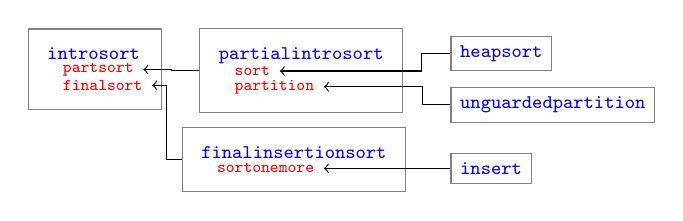
\begin{tikzpicture}[
    node distance=2mm,
%     algoname/.style={font=\fontsize{6}{6}\color{black!50}\ttfamily},
%     depname/.style={rectangle, draw=black!50, font=\scriptsize\ttfamily, anchor=west}
    algoname/.style={font=\scriptsize\color{blue}\ttfamily},
    depname/.style={font=\fontsize{6}{6}\color{red}\ttfamily, anchor=west}
  ]
%     \node (introsort) [algoname] { introsort };
%     \node (introsort-ps) [below=of introsort.west, depname, xshift=2mm] { part\_sort };
%     \node (introsort-fs) [below=of introsort-ps.west, depname] { final\_sort };
%     \node (introsort-box) [draw=black!50, fit={(introsort) (introsort-ps) (introsort-fs)}] {};
%
%     \node (partintrosort) [right=6mm of introsort-box.north east, yshift=-1.15mm, anchor=north west, algoname] { partial\_introsort };
%     \node (partintrosort-s) [below=of partintrosort.west, depname, xshift=2mm] { sort };
%     \node (partintrosort-p) [below=of partintrosort-s.west, depname] { partition };
%     \node (partintrosort-box) [draw=black!50, fit={(partintrosort) (partintrosort-s) (partintrosort-p)}] {};
%
%     \node (insort) [below=2mm of partintrosort-box.south west, anchor=north west, algoname,draw=black!50] { final\_insertion\_sort };
%
%     \node (heapsort) [right=6mm of partintrosort-box.north east, anchor=north west, yshift=-1mm, algoname,draw=black!50] { heapsort };
%     \node (ungrdpart) [below=2mm of heapsort.south west, anchor=north west, algoname,draw=black!50] { unguarded\_partition };
%
%     \draw[->] (heapsort.west) to[-|-=.17] (partintrosort-s.east);
%     \draw[->] (ungrdpart.west) to[-|-=.22] (partintrosort-p.east);
%
%     \draw[->] (insort.west) to[-|-] (introsort-fs.east);
%     \draw[->] (partintrosort-box.west) to[-|-] (introsort-ps.east);

    \node (introsort) [algoname] { introsort };
    \node (introsort-ps) [below=of introsort.west, depname, xshift=2mm] { part\_sort };
    \node (introsort-fs) [below=of introsort-ps.west, depname] { final\_sort };
    \node (introsort-box) [draw=black!50, fit={(introsort) (introsort-ps) (introsort-fs)}] {};

    \node (partintrosort) [right=6mm of introsort-box.north east, yshift=-1.15mm, anchor=north west, algoname] { partial\_introsort };
    \node (partintrosort-s) [below=of partintrosort.west, depname, xshift=2mm] { sort };
    \node (partintrosort-p) [below=of partintrosort-s.west, depname] { partition };
    \node (partintrosort-box) [draw=black!50, fit={(partintrosort) (partintrosort-s) (partintrosort-p)}] {};

    \node (insort) [below=3mm of partintrosort-box.south west, xshift=-1mm, anchor=north west, algoname] { final\_insertion\_sort };
    \node (insort-s) [below=of insort.west, depname, xshift=2mm] { sort\_one\_more };
    \node (insort-box) [draw=black!50, fit={(insort) (insort-s)}] {};


    \node (heapsort) [right=6mm of partintrosort-box.north east, anchor=north west, yshift=-1mm, algoname,draw=black!50] { heapsort };
    \node (ungrdpart) [below=2mm of heapsort.south west, anchor=north west, algoname,draw=black!50] { unguarded\_partition };
    \node (insert) [below=3.85mm of ungrdpart.south west, anchor=north west, algoname,draw=black!50] { insert };

    \draw[->] (heapsort.west) to[-|-=.17] (partintrosort-s.east);
    \draw[->] (ungrdpart.west) to[-|-=.22] (partintrosort-p.east);
    \draw[->] (insert.west) to[-|-=.22] (insort-s.east);

    \draw[->] (insort-box.west) to[-|-] (introsort-fs.east);
    \draw[->] (partintrosort-box.west) to[-|-] (introsort-ps.east);
  \end{tikzpicture}
  \caption{Modular verification of Introsort. The boxes show the different
    algorithms and the specifications they depend on. Arrows point from an algorithm to the specification that it implements.}\label{fig:modular}
  \end{figure}

  % TODO: Despite this explicit modularization, we also do implicit modularization, by inserting concrete algorithms
  %  early, but only using their spec for the correctness proof

\subsection{Unguarded Insertion Sort}\label{sec:unguarded_insort}
  We also use refinement for the implementation of insertion sort.
  As suggested in the pseudocode (Alg.~\ref{alg:insort}), we use a Boolean variable to discriminate
  between the guarded and unguarded versions. Only in the last refinement step we will specialize the algorithm for both cases.

  For the correctness proof, we first specify insertion as sorting one more element of an already sorted list:
  \begin{lstlisting}
    sort_one_more_spec G xs i ==
      assert (i<|xs| \and sorted (xs[0..<i]));
      assert (\<not>G --> 0<i \and \<not>(xs[i] < xs[0]));
      spec xs'. inres (slice_sort_spec xs 0 (i+1)) xs'
                \and (\<not>G --> xs'[0] = xs[0]))
  \end{lstlisting}
  Assuming the initial segment of the list up to \is{i} is already sorted,
  afterwards, the segment up to \is{i+1} will be sorted, and the rest of the list
  will be unchanged. We reuse \is{slice_sort_spec} for this (\is{inres m x} states that \is{x} is a possible result of \is{m}).
  In the unguarded case (\is{\<not>G}), we assume that the first element of the list to be sorted is not greater than
  the element to be inserted, which guarantees that insertion will stop latest at this element. Moreover, we explicitly guarantee
  that the first element of the list will not change\footnote{This is stronger than required, as in the general case of weak orderings,
  it would be fine to exchange the first element by an equivalent one. However, it holds for our implementation and slightly simplifies the proofs.}.

  Using this specification, and its canonical refinement to slices, it is straightforward to prove correct the final
  insertion sorting algorithm (cf.~Alg.~\ref{alg:insort}). We now focus on the actual insertion procedure.
  In a first step, we refine the specification to a version that describes what the insertion procedure actually does,
  rather than focusing on the sorting:
  \begin{lstlisting}
    insert_spec G xs i ==
      assert (i<|xs| \and (\<not>G --> 0<i \and \<not>(xs[i] < xs[0])));
      spec xs'. \<exists>i'<=i.
        xs'=xs[0..<i'] @ xs[i] @ xs[i'..<i] @ xs[i<${}$..]
      \and \<forall>j\<in>{i'<${}$..i}. xs[i] < xs'[j]
      \and i'>0 --> \<not>(xs[i] < xs'[i'-1])
      "
  \end{lstlisting}
  This precisely describes how the element at index \is{i} is moved backwards over greater elements.
  Its new index is \is{i'}, and if this is not the beginning of the list, the element at \is{i'-1} was not greater,
  such that the moving could be stopped.

  This specification refines \is{sort_one_more_spec}:
  \begin{theorem}
  \begin{lstlisting}
    insert_spec xs i <= sort_one_more_spec xs i
  \end{lstlisting}
  \end{theorem}
  The proof requires some basic arguments about relating equalities on list indices to equalities on lists and sets.
  Although straightforward in principle, it required a few auxiliary lemmas.
  Again, refinement allows us to do this reasoning in isolation, and then focus on how to implement the moving
  of the element.

  We implement the insert procedure on whole lists first, and then refine it to slices beginning at index \is$l$.
  We only display the version on slices here:
  \begin{lstlisting}
    slice_insert G xs l i ==
        x <- xs[i];
        (xs,i) <- while$_I$ (\<lambda>(xs,i). (\<not>G \or i>l) \and x<xs[i-1]) (\<lambda>(xs,i).
            xs <- xs[i:=xs[i-1]]
            return (xs,i-1) ) (xs,i)
        xs <- xs[i:=x]
        return xs
  \end{lstlisting}
%
%   In a second refinement step, the algorithm is refined to work on slices of lists
%
%
%
%
%   The insertion algorithm resembles the one displayed in Alg.~\ref{alg:insort}:
%   \begin{lstlisting}
%     insert G xs i ==
%         x <- xs[i];
%         (xs,i) <- while$_I$ (\<lambda>(xs,i). (\<not>G \or i>0) \and x<xs[i-1]) (\<lambda>(xs,i).
%             xs <- xs[i:=xs[i-1]]
%             return (xs,i-1) ) (xs,i)
%         xs <- xs[i:=x]
%         return xs
%   \end{lstlisting}
  As this is a functional program, the variables \is{xs} and \is{i} have to be threaded through the loop explicitly.
  Moreover, instead of updating a single index, we update the whole list and rebind the updated list to the same name as
  the old list (\is{xs <- xs[i:=x]}). Finally, the loop is annotated with an invariant $I$. It is completely standard
  and not displayed here.

  We easily prove that \is{slice_insert} refines \is{slice_insert_spec}, and, by transitivity,
  it also refines \is{slice_sort_one_more_spec}. Thus, we can plug it into the insertion sort algorithm, which, in turn, is plugged into the main Introsort algorithm (cf.\ Fig.~\ref{fig:modular}).


\subsection{Heapsort and Partition}
  \newcommand{\leftc}{\textrm{left}}
  \newcommand{\rightc}{\textrm{right}}

  The proofs of heapsort and partitioning follow a similar plot, and are not displayed here in full.
  We used some existing Isabelle proofs as guideline \cite{LaWi19-IMP2,Gri19-AFP,La16}.
  However, we point out one more interesting application of refinement: recall the sift-down function on heaps,
  that restores the heap property by \emph{floating down} an element\footnote{see, e.g., \cite[Ch.~6]{CLRS09} or \cite[Ch.~2.4]{SeWa11} for a description of heapsort.}. Usually, this function is presented by swapping the element with one of its children, until the heap property is restored (Alg.~\ref{alg:sift_down_swap}).
  \begin{algorithm}
    \begin{algorithmic}
    \Procedure{sift\_down}{$a,i$}
      \While{has right child $i$}
        \If{$a[\leftc~i] < a[\rightc~i]$}
          \If{$a[i] < a[\rightc~i]$}
            \State{\Call{swap}{$a[i], a[\rightc~i]$}}
            \State{$i\gets \rightc~i$}
          \Else~\Return{}
          \EndIf
        \ElsIf{$a[i] < a[\leftc~i]$}
          \State{\Call{swap}{$a[i], a[\leftc~i]$}}
          \State{$i\gets \leftc~i$}
        \Else~\Return{}
        \EndIf
      \EndWhile
      \If{has left child $i$ and $a[i] < a[\leftc~i]$}
        \State{\Call{swap}{$a[i], a[\leftc~i]$}}
      \EndIf
    \EndProcedure
    \end{algorithmic}
  \caption{Pseudocode of sift-down function with swap}\label{alg:sift_down_swap}
  \end{algorithm}
  \begin{algorithm}
    \begin{algorithmic}
    \Procedure{sift\_down\_opt}{$a',i$}
      \State{$t\gets a'[i]$}
      \While{has right child $i$}
        \If{$a'[\leftc~i] < a'[\rightc~i]$}
          \If{$t < a'[\rightc~i]$}
            \State{$a'[i]\gets a'[\rightc~i]$}
            \State{$i\gets \rightc~i$}
          \Else~\Return{}
          \EndIf
        \ElsIf{$t < a[\leftc~i]$}
          \State{$a'[i]\gets a'[\leftc~i]$}
          \State{$i\gets \leftc~i$}
        \Else~\Return{}
        \EndIf
      \EndWhile
      \If{has left child $i$ and $t < a'[\leftc~i]$}
        \State{$a'[i]\gets a'[\leftc~i]$}
        \State{$i\gets \leftc~i$}
      \EndIf
      \State{$a'[i]\gets t$}
    \EndProcedure
    \end{algorithmic}
  \caption{Pseudocode of optimized sift-down function}\label{alg:sift_down_opt}
  \end{algorithm}
  However, the element that is written to $a[\rightc~i]$ or $a[\leftc~i]$ by the swap will get overwritten in the next loop iteration.
  Thus, a common optimization to save half of the writes is to store the element to be moved down in a temporary variable, and only
  assign it to its final position after the loop (Alg.~\ref{alg:sift_down_opt}). Note that the insertion procedure of insertion sort does a similar optimization.
  However, for the insertion procedure, it was feasible to prove the optimization together with the actual algorithm.
  For the slightly more complicated sift-down procedure, we first prove correct the simpler algorithm with swaps,
  and then refine it to the optimized version. Inside the loop, the refinement relation between the concrete array \is{a'} and the
  abstract array \is{a} states that
  we obtain \is{a} as \is{a'[i:=t]}. The proof that the optimized version refines the version with swaps requires only about 20
  lines of straightforward Isabelle script.


\section{Imperative Implementation}
  In the previous sections, we have presented a refinement based approach to verify the Introsort algorithm,
  including most optimizations we found in its GNU C++ Library implementation. However, the algorithm is still expressed
  as a nondeterministic monadic program that modifies functional lists. In this section, we discuss how the Isabelle LLVM framework~\cite{La19-llvm} is
  used to (semi-)automatically transfer the algorithm into an LLVM program on arrays.

  \subsection{The Sepref Tool}
  The idea of the Sepref tool~\cite{La15,La19-llvm} is to symbolically execute an abstract program in the \is{nres}-monad,
  keeping track of refinements of every abstract variable to a concrete representation that may use pointers to dynamically allocated memory.
  During this symbolic execution, the tool can synthesize an imperative program in the Isabelle-LLVM semantics, together with a refinement proof.
  The tool works automatically, but usually requires some program-specific setup and boilerplate. For a detailed discussion of the Sepref tool and the Isabelle-LLVM framework, we refer the reader to~\cite{La15,La19-llvm}.

  Isabelle-LLVM comes with standard setup to refine lists to arrays. List update operations are refined to destructive array element updates,
  as long as the old version of the abstract list is not used any more after the update. Note that, by rebinding the updated list to the same
  variable name as the original list\footnote{as e.g.\ in \is{xs <- xs[i:=x]}, cf.\ Sec.~\ref{sec:unguarded_insort}}, this property is syntactically ensured. Moreover, Isabelle-LLVM provides setup to refine the unbounded integers of Isabelle/HOL to bounded integers.
  The resulting proof obligations to show that the integers are in bounds are discharged automatically, but typically require some hinting from the user.
  A common technique to provide such hints is to insert additional assertions into the abstract program.
  Usually, these can be proved easily. For example, in the definition of \is{slice_partial_introsort} (Sec.~\ref{sec:refinement}),
  we have inserted the assertion \is{l<=h} at the very beginning. This is required by the Sepref tool to prove that the operation \is{h-l}
  in the next line cannot underflow. This assertion adds a proof obligation to the proof that \is{slice_partial_introsort} refines \is{slice_part_sort_spec} (Thm.~\ref{thm:slice_partial_introsort_correct}), which is, however, trivial, as the specification
  explicitly states \is{l<=h} as precondition. On the other hand, when refining \is{slice_partial_introsort} to an implementation with bounded
  integers, one can assume \is{l<=h}, thus discharging the non-underflow proof obligation for the \is{h-l} operation.
  Thus, assertions provide a convenient tool to pass properties down the refinement chain.

  Using the Sepref tool, it is straightforward to refine the Introsort algorithm to an Isabelle-LLVM program that sorts arrays of integers.
  For example, Figure~\ref{fig:ug_insort_isa_llvm} shows the Isabelle-LLVM code that is generated for the \is{insert} procedure with \is{G=false} (cf.~\ref{sec:unguarded_insort}).
  Moreover, the Sepref tool will generate a theorem that the generated program actually implements the abstract one:
  \begin{theorem}
    \begin{lstlisting}
      (ug_insert_impl, slice_insert False)
        : arr_u64$^d$ \x snat64$^k$ \x snat64$^k$ -> arr_u64
    \end{lstlisting}
  \end{theorem}
  This specifies the relations for the parameters and the result, where \is{arr_u64} relates arrays of unsigned 64-bit integers with lists of integers,
  and \is{snat64} relates non-negative 64-bit integers with natural numbers.
  The $\cdot^d$ annotation means that the parameter will be \emph{destroyed} by the function call,
  while $\cdot^k$ means that the parameter is \emph{kept}.
  Here, the insertion is done in place, such that the input list has no corresponding refinement after the function call.

  The final correctness statement for our Introsort implementation (for integers) is
  \begin{theorem}
    \begin{lstlisting}
      (introsort_impl, slice_sort_spec)
        : arr_u64$^d$ \x snat64$^k$ \x snat64$^k$ -> arr_u64
    \end{lstlisting}
  \end{theorem}
  Here, \is$introsort_impl$ is the Isabelle-LLVM program generated by Sepref from \is$introsort$ (cf.\ Sec.\ \ref{sec:refinement}).
  This theorem combines the refinement theorem generated by Sepref, and Theorem~\ref{thm:introsort_correct}.

  \begin{figure}
    \begin{lstlisting}
      ug_insert_impl == %xs l i. doM {
          x <- array_nth xs i;
          (xs, i) <- llc_while (%(xs, i). doM {
              bi <- ll_sub i 1;
              t <- array_nth xs bi;
              ll_icmp_ult x t
          }) (%(xs, i). doM {
              i' <- ll_sub i 1;
              t <- array_nth xs i';
              xs <- array_upd xs i t;
              i <- ll_sub i 1;
              return (xs, i)
          }) (xs, i);
          array_upd xs i x
        }
    \end{lstlisting}
    \caption{Implementation for \is{insert} procedure with \is{G=false} generated by the Sepref tool, for 64bit signed integer elements.
      This definition is within the executable fragment of Isabelle-LLVM, i.e.,
      the Isabelle LLVM code generator can, after preprocessing, translate it to LLVM-IR. Moreover, note that the function does not
      depend on the lower bound parameter \is$l$ any more, as this was only required in the guarded version.
    }\label{fig:ug_insort_isa_llvm}
  \end{figure}

  \begin{figure}
    \begin{lstlisting}[language=llvm,literate={}]
      define i64* @ug_insert_impl(i64* %xs, i64 %l, i64 %i) {
      start:
        %x3 = getelementptr i64, i64* %xs, i64 %i
        %r = load i64, i64* %x3, align 8
        br label %while_start

      while_start:
        %bib.sink = phi i64 [ %bib, %while_body ], [ %i, %start ]
        %bib = add i64 %bib.sink, -1
        %xda = getelementptr i64, i64* %xs, i64 %bib
        %ra = load i64, i64* %xda, align 8
        %xg = icmp ult i64 %r, %ra
        %p1 = getelementptr i64, i64* %xs, i64 %bib.sink
        br i1 %xg, label %while_body, label %while_end

      while_body:
        store i64 %ra, i64* %p1, align 8
        br label %while_start

      while_end:
        store i64 %r, i64* %p1, align 8
        ret i64* %xs
      }
    \end{lstlisting}
    \caption{LLVM-IR generated by Isabelle-LLVM for the definition from Figure~\ref{fig:ug_insort_isa_llvm}.
    We display the code after an LLVM optimization pass that eliminates some redundant operations generated by Isabelle-LLVM,
    and thus makes the code more readable. Note that we kept the unused parameter \%l. LLVM will eliminate it by inlining the function.
    }\label{fig:ug_insort_llvm}
  \end{figure}

  \subsection{The Isabelle-LLVM Code Generator}
  Isabelle-LLVM comes with a code generator that exports this program to actual LLVM text, which is subsequently compiled using the LLVM toolchain.
  Fig.~\ref{fig:ug_insort_llvm} shows the code generated for the \is{slice_insert} procedure.


  To make the generated programs usable, one has to link them to C wrappers, that handle parsing of command line options and printing of results.
  However, the original Isabelle-LLVM framework provides no support for this: one has to manually write a C header file, that hopefully matches the object file generated by the LLVM compiler. If it doesn't, the program has undefined behaviour\footnote{In practice, this means it will probably SEGFAULT. However, it also might return wrong results, or be prone to various kinds of exploits.}. What makes the situation even worse is, that the C compiler sometimes changes function signatures: For example, a function with a non-primitive return value (e.g. a structure) is changed to a void function with an extra
  reference parameter for the return value. LLVM, on the other hand, does not perform this change, which makes the function generated by LLVM incompatible with the function call generated by the C compiler.

  To this end, we extended Isabelle-LLVM to also generate a header file for the exported functions, refusing to export functions whose signatures
  would be altered by the C compiler. Figure~\ref{fig:export} shows the extended Isabelle LLVM export command and the generated header file for our Introsort algorithm on strings.
  \begin{figure}
    \begin{flushleft}\bfseries\color{black!50} Isabelle command\end{flushleft}
    \begin{lstlisting}
      export_llvm
        str_sort_introsort_impl
          is llstring* str_introsort(llstring*, int64_t, int64_t)
        defines \<open>
          typedef struct {
            int64_t size; struct {int64_t capacity; char *data;};
          } llstring; \<close>
    \end{lstlisting}
    \medskip

    \begin{flushleft}\bfseries\color{black!50} Generated C header\end{flushleft}
    \begin{lstlisting}[language=C]
      typedef struct {
        int64_t size;
        struct {
          int64_t capacity;
          char*data;
        };
      } llstring;

      llstring* str_introsort(llstring*, int64_t, int64_t);
    \end{lstlisting}

    \caption{An example Isabelle command to export LLVM code for a string sorting function, and the generated header file.
    Strings are represented as dynamic arrays of characters.
    Isabelle will refuse to export functions whose signatures
    would be changed by C. Moreover, structure fields in LLVM are indexed by consecutive numbers, rather than named by meaningful names.
    Our extension allows to define properly named structures for the header file, and checks that these definitions are actually compatible with
    the LLVM signatures.
    }\label{fig:export}
  \end{figure}

  \subsection{Separation Logic and Ownership}
  Internally, the Sepref tool represents the symbolic state, which contains all abstract variables and their refinements to concrete variables,
  as an assertion in separation logic~\cite{Rey02,CHY07}. For example, the assertion
  \begin{lstlisting}
    array xs_1 p_1 * array xs_2 p_2
  \end{lstlisting}
  describes a symbolic state that refines the two abstract list variables \is{xs_1} and \is{xs_2} by
  two arrays at addresses \is{p_1} and \is{p_2}. Separation logic guarantees that the arrays at \is{p_1} and \is{p_2}
  share no common memory, i.e.,
  updates to the first array cannot change the second array. As long as the array elements are
  primitive values like integers, this works as expected, and a list of integers can be refined
  to an array of integers. An array lookup operation will simply return a copy of the integer
  value at the specified index. It can be specified by the following Hoare-triple, which can
  be used by Sepref to synthesize LLVM code for the operation \is{r <- xs[i]}.
  \begin{lstlisting}
    { array xs p * i<|xs| } r = p[i] { array xs p * r=xs[i] }
  \end{lstlisting}
  Note that we use C like notation for the program, and abstracted away the fact that the \is{i}
  in the program is a bounded integer register from LLVM, while the \is{i} in the assertions refers to
  its content as an unbounded Isabelle integer.

  Now, let's assume we have a list of strings, where a string is itself a list of characters.
  The following assertion refines both, the outer and the inner lists to arrays:
  \begin{lstlisting}
    sarray xs p == \<exists>ys.
      |ys|=|xs| * array ys p * array xs_1 ys_1 * ... array xs$_n$ ys$_n$
  \end{lstlisting}
  Here, \is{ys} represents the list of string pointers, which point to their own separate array each.
  The canonical Hoare triple for array lookup would be:
  \begin{lstlisting}
    { sarray xs p * i<|xs| } r = p[i] { sarray xs p * array (xs[i]) r }
  \end{lstlisting}
  However, this does not hold, as the inner array at position \is{i} is now pointed to twice:
  by \is{r} and by the \is{ys[i]} from within the \is{sarray} assertion. The only way to make a
  Hoare triple of this form valid is to make a copy of the inner array, which would come with an
  unacceptable performance penalty.

  The Rust Programming Language~\cite{rustlang} has to solve a similar problem.
  There, they use the concept of borrowing: the inner array is \emph{borrowed} from the outer one,
  i.e., ownership is transferred to the variable \is{r}. Only at the end of the lifetime of \is{r},
  ownership will return to the outer array\footnote{Actually, borrowing in Rust does not work for array elements,
  as the type-checking would become undecidable. Fortunately, in an interactive theorem prover, we can burden the
  user with parts of this type checking.}. We realize a similar concept in Sepref, by refining abstract lists of
  optional values to arrays, that only own those elements which are present (not None) in the abstract list\footnote{For simplicity, the presentation sticks to the array of strings example. Actually, our implementation is parameterized over the refinement for the inner type.
  We believe that a further generalization to include outer types other than lists (e.g.\ maps) is possible, but leave it for future work.}:
  \begin{lstlisting}
    oarray xs p == \<exists>ys. array ys p * A' xs_1 ys_1 * ... * A' xs$_n$ ys$_n$
    $\textrm{where }$
    A' None _ = \<box>  |  A' (Some x) y = array x y
  \end{lstlisting}
  We define abstract operations to borrow and return (insert) elements, as well as to convert between a
  standard list and a list with explicit ownership:
  \begin{lstlisting}
    borrow xs i == assert (i<|xs| \and xs[i]~=None);
                  return (the (xs[i]), xs[i:=None])
    ins xs i x == assert (i<|xs| \and xs[i]=None);
                  return xs[i:=Some x]
    to_olist xs = return (map Some xs)
    to_slist xs = assert (None \<notin> xs); return (map the xs)
  \end{lstlisting}
  Here, \is{the (Some x) = x} is the selector function of the option data type.
  The \is{borrow} function assumes that the element is still present in the list, and then returns the element
  and a new list where the element is gone. Symmetrically, the \is{ins} function assumes that there is no element
  present at the specified index. The \is{to_olist} and \is{to_slist} functions convert between lists of plain values and lists
  of optional values, where \is{to_slist} assumes that all values in the list are actually present.

  This approach allows us to explicitly model ownership transfer of array elements in the \is{nres} monad, and let Sepref
  generate efficient code, sparing explicit copies of elements.

  The necessary conversion operations can usually be inserted by a straightforward refinement step.
  For example, we refine the \is{insert} function (Sec.~\ref{sec:unguarded_insort}) as follows:
  \begin{lstlisting}
    is_insert_o G xs' i ==
      xs' <- to_olist xs';
      (x,xs') <- borrow xs' i;
      (xs',i) <- while
        (%(xs',i). (\<not>G \or i>0) \and xs' < xs'[i-1]) (%(xs',i).
          (t,xs') <- borrow xs' (i-1);
          xs' <- ins xs' i t;
          return (xs', i-1)
        ) (xs',i);

      xs' <- ins xs' i x;
      return (to_slist xs')
    }
  \end{lstlisting}
  First, this function converts the input list \is{xs'} to one with explicit ownership.
  It then borrows the element \is{i} from this list. In each loop iteration, it moves an element
  from \is{i-1} to \is{i}, by borrowing and immediately re-inserting it.
  Finally, the element borrowed at the beginning is re-inserted, and the list is converted back to implicit ownership.
  The refinement proof is, again, straightforward. The refinement relation for the loop states that the abstract and concrete array
  contain the same values, except at index \is{i}, where the concrete value is not present:
  \begin{lstlisting}
    |xs'| = |xs|
    \and (\<forall>j<|xs|. j~=i --> xs'[j] = Some (xs[j])) \and xs'[i]=None}
  \end{lstlisting}


  Using this explicit ownership extension to Sepref, we can also synthesize the Introsort algorithm for arrays of arrays of characters,
  where the inner arrays are compared lexicographically.


%   xxx, ctd here: Define slice_partition_spec the same way! Then show refinement of algo!
%     lemma "partition3_spec xs l h = ⇓(slice_rel xs l h ×⇩r Id) (doN { ASSERT (h-l≥4 ∧ h≤length xs); (xs⇩1,xs⇩2) ← partition1_spec (slice l h xs); RETURN (xs⇩1@xs⇩2, l+length xs⇩1) })"
%
%
%
%   xxx, ctd here: slicep_rel and slice_rel. Do we need two steps?
%
%




\section{Benchmarks}
  The goal of this paper was to verify
  an existing real-world implementation of a medium-complex algorithm.
  We chose the Introsort implementation from the GNU C++ library. As we did not directly verify the existing C++ code,
  but re-implemented the algorithm using Isabelle-LLVM, we have to test how close we came to the performance of the original.

  Our benchmark set is based on the Boost C++ Library's~\cite{boost} sorting algorithm benchmarks, extended with further benchmarks indicated in~\cite{Bent93}.
  Apart from sorting a random list of elements that are mostly different (random), we also sort lists of length $n$ that contain only $n/10$ different elements (random-dup-10), and random lists of only two different elements (random-boolean), as well as lists where all elements are equal (equal).
  We also consider already sorted sequences (sorted, rev-sorted), as well as a sequence of $n/2$ elements in ascending order, followed by the same elements in descending order (organ-pipe). We also consider sorted sequences where we applied $pn/100$ random swap operations (almost-sorted-$p$).
  Finally, we consider sorted sequences with $pn/100$ random elements inserted at the end or in the middle ([rev-]sorted-end-$p$, [rev-]sorted-middle-$p$).

  We sorted integer arrays with $n=10^8$ elements, and string arrays with $n=10^7$ elements.
  To represent strings, we used dynamic arrays of characters, and used the same compare function for our algorithm and std::sort,
  in order to eliminate differences in the compare function implementation\footnote{Initially, we used std::string elements for std::sort,
  for which the compare function seems to be significantly slower than our compare function on dynamic arrays.}.

  We compile both, our verified algorithm and the std::sort benchmark with clang-6.0.0.
  The benchmarks were run on a laptop with an Intel(R) Core(TM) i7-8665U CPU and 32GiB of RAM, as well as on a server machine with
  24 AMD Opteron 6176 cores and 128GiB of RAM. Ideally, the sorting algorithm should take exactly the same time when run on the same data and machine.
  However, in practice, we encountered some noise. We encountered both, \emph{high frequency} noise, that slowed down single sorting
  runs, and \emph{low frequency} noise, that slowed down the machine for several minutes. To counter the high-frequency noise,
  we ran each experiment 10 times in a row, dropped the 6 extremal results, and report the average of the remaining 4 results.
  If the smallest remaining result was more than 2\% smaller than the largest remaining result, we repeated the experiment.
  Countering the low-frequency noise is more time consuming. For all benchmarks, we repeated the slower experiment when the
  difference between our algorithm and std::sort was more than 15\%\footnote{The outlier for sorted-end-1 on the server machine seems to be genuine. We have no explanation for that.}. Moreover, for the random and organ-pipe integer benchmarks,
  we ran all the experiments in a loop for several hours, and report the intervals of the averages of the median 4 values.
  The results are displayed in Tables~\ref{tab:benchmarks} and ~\ref{tab:bench_longrun}.

  \begin{table}{\footnotesize
    \begin{tabular}{|l|S|S||S|S|}
      \hline
      \multirow{2}{*}{Data Set}&\multicolumn{2}{c||}{uint64}&\multicolumn{2}{c|}{llstring}\\
      & Lap & Srv & Lap & Srv \\
      \hline
      random & -0.5 & 2.4&-14.5 & -2.1\\
      random-dup-10 & -0.2 & 3.2&-1.2 & -1.7\\
      random-boolean & -0.1 & -0.7&4.7 & 5.3\\
      equal & -13.3 & 0.9&6.9 & 4.0\\
      sorted & 6.6 & 3.0&2.2 & 4.2\\
      rev-sorted & 1.9 & 3.8&2.1 & 2.0\\
      organ-pipe & -8.1 & 12.8&7.0 & 4.9\\

      almost-sorted-10 & 3.8 & 1.3&-0.8 & -2.0\\
      almost-sorted-.1 & 3.2 & 1.7&2.3 & -0.7\\
      almost-sorted-1 & -8.7 & 2.2&-11.1 & -1.1\\
      almost-sorted-50 & -0.0 & 2.5&-12.2 & -1.8\\

      sorted-end-10 & -4.3 & 1.3&-1.0 & -1.4\\
      sorted-end-.1 & -4.0 & 8.3&-4.7 & 11.9\\
      sorted-end-1 & -5.2 & 19.9&10.4 & 5.6\\
      sorted-middle-10 & -1.1 & 3.2&-0.7 & -2.7\\
      sorted-middle-1 & 12.5 & 4.5&5.4 & 2.1\\
      sorted-middle-.1 & -2.8 & 4.4&6.1 & 6.6\\

      rev-sorted-end-10 & 1.1 & 3.1&-1.5 & -2.4\\
      rev-sorted-end-.1 & 5.6 & 8.7&0.9 & 5.4\\
      rev-sorted-end-1 & 9.7 & 3.9&-12.6 & 0.6\\
      rev-sorted-middle-10 & 1.2 & 6.2&-14.3 & -0.6\\
      rev-sorted-middle-1 & -2.3 & 3.6&-12.0 & 0.9\\
      rev-sorted-middle-.1 & -5.7 & 4.2&3.4 & 5.5\\
      \hline
    \end{tabular}}
    \caption{Benchmark results, as the ratio $(i/c - 1)*100$, where $i$ and $c$ are the average wall-times of verified Introsort and std::sort.
    That is, negative values indicate that Introsort was faster, and positive values indicate that std::sort was faster.
    }\label{tab:benchmarks}
  \end{table}
  \begin{table}\footnotesize
    \begin{tabular}{|l|SSS|SSS|}
      \hline
      \multirow{2}{*}{Algorithm} & \multicolumn{3}{c|}{random} & \multicolumn{3}{c|}{organ-pipe} \\
      & {min} & {max} & {r} & {min} & {max} & {r} \\
      \hline
      isabelle::sort &7.35 & 8.58 & 16.7 & 8.43 & 9.86 & 17.0 \\
      std::sort &7.38 & 8.63 & 17.0 & 8.97 & 10.49 & 16.9 \\
      \hline
    \end{tabular}

    \caption{Intervals of the results (wall time in seconds) for repeating each experiment 74 times,
      in an interleaved fashion. The $r$ fields display $(\max/\min-1)*100$, i.e., the value that
      would appear in Table~\ref{tab:benchmarks} when comparing the slowest and fastest run of the same experiment.
      }\label{tab:bench_longrun}
  \end{table}

  The results clearly show that our verified sorting algorithm performs on-par with the GNU C++ Library's implementation,
  within the expected noise of up to $17\%$. Table~\ref{tab:bench_longrun} even indicates that our algorithm performs
  slightly better on our laptop machine. We leave it to future work to do more precise measurements on different machines.

%   \subsection{Proof Architecture of Introsort}
%     Start with introsort-scheme. Motivate stepwise refinement "in the small" to get
%     from list-concatenation to slicing.
%
%     Then illustrate big-picture architecture. Mention that we use similar "in the small" techniques for other modules.
%
%     Finally show how final algorithm is assembled (nres-level)
%
%     THEN introduce sepref tool, and illustrate how final algorithm is refined, module by module.
%     mention parameterization over sort function.
%
%     Can we motivate the array-ownership stuff?
%
%
%
%
% \section{Isabelle-LLVM}
%   Quick intro to Isabelle-LLVM
%
%   \subsection{Nested Containers and Ownership}
%     Our prototype solution
%     Rust's ownership model
%     Outlook: Fractional separation logic for read-only borrowing
%     Still unsolved: Abstractly immutable, but concrete mutations
%       (E.g. union-find with path compression, amortized search-trees?) Invalid in concurrent setting, but perfectly OK in sequential setting!
%
%
%
%   \subsection{Isabelle-LLVM Code Generator}
%   Small TCB.
%
%
% \section{Verification of Introsort}
%
%   Layout general architecture (Quicksort-Scheme)
%   Main proof steps and concepts:
%     Partially sorted
%     Guards
%     Plugging together the implementation
%
%
%   Observations
%     sledgehammer tool is really useful. But prone to not properly abstract/modularize the proofs,
%       which will only work until sledgehammer can't solve a goal. At this point, usually
%       refactoring of the whole proof is required to make it manageable again.
%
%
%
%
% \section{Benchmarks}
%   64 bit integers,
%   character arrays (we don't have a std::string implementation in Isabelle-LLVM yet)
%
%   benchmark suite taken from BOOST. Added some more test cases from Timsort(?) paper.
%
%
%   Benchmark the heapsort-algorithm alone!
%
%
%   Add Test:
%     Organpipe  123..nn.. 321
%     Random 0-1 arrays



\section{Conclusions}
In this paper we have verified the state-of-the art Introsort sorting algorithm using Isabelle-LLVM.
We included most optimizations found in the GNU C++ Library's (libstdc++) implementation.
On an extensive set of benchmarks, our verified implementation performs on par with the libstdc++ implementation.

The verification took us about 100 person hours distributed over 4 weeks. After two weeks and roughly 60 person hours,
we had arrived at an algorithm that was only about 10\% slower than std::sort. However, it only worked for integers, and always
used guarded insertion sort. The remaining time was spent on implementing explicit ownership for Sepref, such
that we could sort strings and other objects, and on verifying the unguarded insertion sort optimization.


% Verification Effort: ca 100 person-hours, including benchmarking and extension of Isabelle-LLVM to support nested containers.
% ca 60 person-hours to arrive at first integer sorting algorithm that was competitive [this time, however, includes heapsort implementation, which is not strictly necessary for competitive algorithm, but was done quite early in the project].
% XXX lines of proof.


This shows that Isabelle-LLVM can be used to generate competitive verified implementations of medium-complex algorithms.
The Refinement Framework has been successfully used for much larger projects, e.g., model-checkers~\cite{ELNN13,BrLa18,WiLa18}.
However, these developments produce implementations that use arbitrary precision integers and target Standard ML,
which means a principal performance deficit compared to more low-level implementations. Using Isabelle-LLVM as backend to the Refinement Framework,
these limitations can now be overcome. Thanks to the modular structure of the Refinement Framework, we can even hope to gradually
transform existing verification projects to Isabelle-LLVM, e.g., replacing invocations of functional mergesort on lists by
our Introsort algorithm on arrays in a first step.

While we can easily instantiate our sorting algorithm to arbitrary weak orderings on arbitrary element types \emph{within} the Refinement Framework,
we cannot so easily replace C++'s std::sort. The reason is that std::sort is a template which is instantiated by the C++ compiler,
i.e., before LLVM intermediate code is even generated. Verifying the std::sort template itself would require a formal semantics of C++,
including its template mechanism and the relevant traits from the standard template library (orderings, iterators, etc.). To the best of our knowledge, such a semantics has not yet been formalized, let alone being used to verify non-trivial algorithms.
However, we can \emph{specialize} the std::sort template to use our Introsort algorithm for any fixed combination of element type and ordering, on containers backed by an array (e.g.\ std::vector).

Finally, the trusted code base of Isabelle-LLVM is relatively small, even compared to other common program verification methods.
Following the LCF tradition~\cite{gordon-et-al-1979}, the Isabelle prover is designed around a small inference kernel, which is the only code
whose bugs can affect the correctness of proved theorems.
The Isabelle-LLVM framework contains a relatively straightforward formalization of the LLVM semantics, with a straightforward code
generator~\cite{La19-llvm} to LLVM intermediate language.
Finally, the LLVM compiler is an industrial strength, well-tested, and widely used compiler.
In contrast, the default code generators of most theorem provers target high level languages, which includes the
compilers and the high-level language semantics into the trusted code base.
Deductive verification tools like KeY~\cite{BHS07} depend on the correct axiomatization of the highly complex Java semantics,
as well as on several automatic theorem provers, which, themselves, are highly complex and optimized C programs.

To reduce the trusted code base even further, one can include a compiler correctness proof in the theorem prover:
The Verifiable C project~\cite{App14} provides a verification infrastructure on top of the verified CompCert compiler~\cite{BL09}.
However, to the best of our knowledge, this has only been applied to verify rather simple programs~\cite{CBGD18}.
The CakeML project \cite{KTMK19,MyOw14} has developed a code generator for HOL4 and a verified ML compiler.
However, the performance of functional high-level languages seems to be inherently limited wrt.\ low-level imperative languages,
and we are not aware of any high-performance algorithm that has been verified using CakeML.


\subsection{More Related Work}
Sorting algorithms are a standard benchmark for program verification tools, such that we cannot give an exhaustive overview.
Nevertheless, we discuss a few notable examples: The arguably first formal proof of quicksort was given
by Foley and Hoare himself~\cite{FoHoa71}, though, due to the lack of powerful enough theorem provers at these times,
it was only done on paper.

One of the first mechanical verifications of imperative sorting algorithms is by
Filli{\^a}tre and Magaut~\cite{FiMa99}, who prove correct imperative versions of quicksort, heapsort, and insertion sort in Coq.
However, they do not report on code generation or benchmarking, nor do they combine their separate algorithms to Introsort.

The Timsort algorithm, which was used in the Java standard library, has been verified
with the KeY tool~\cite{GRBBH15}. A bug was found and fixed during the verification.
Subsequently, KeY has been used to also verify the dual-pivot quicksort algorithm from the
Java standard library~\cite{BSSU17}. This time, no bugs were found.

\subsection{Future Work}
Actually, the C++ standard requires the std::sort algorithm to not only be functional correct,
but to also have a worst-case complexity of $O(n\log n)$. Recently, the Refinement Framework has been extended to reason
about time complexity~\cite{HaLa19}, and it has been proposed that Isabelle-LLVM could be used as a backend.
This would enable us to also formally prove the worst-case complexity of Introsort.

Another obvious direction is to formalize other state-of-the-art implementations of sorting algorithms,
for example std::stable\_sort, or Boost's pattern defeating quicksort~\cite{boost} with branch prediction optimization~\cite{EdWe16}.

Finally, we proposed an explicit ownership model for nested lists.
However, we only support write-ownership. A next step would be to include read-ownership, which allows aliasing on read-only objects.
Formally, this could be realized with fractional permissions~\cite{BCOP05}.


%
% Future work:
%   Proof complexity (Use refinement-with-time)
%   More optimizations (eg PD-Qsort)
%   Specialized algorithms for integers and strings (radix sort, burstsort, etc ... -> Boost library)


\paragraph{Acknowledgements}Hidden for blind review.
%
% We received funding from DFG grant LA 3292/1 "Verifizierte Model Checker" and VeTSS grant "Formal Verification of Information Flow Security for Relational Databases".


%
%
% The Compcert project~\cite{compcert} has formalized a correct compiler for C to machine code
%
% This has been done in Coq for a fragment of the C language
%
%
%
% Most other algorithms that are verified with interactive theorem provers such as Isabelle, Coq~\cite{XX}, or ACL2 \cite{XX}
%
%
% xxx: CompCert, CakeML --> actually smaller code-base
%
%
%
%
% Apart from the obvious things such as the machine and operating system,
% and the Theorem Provers kernel
%
%
%
%
%
%
%
%
%
%
%   As our verification targets LLVM, we cannot directly replace std::sort, which is a C++ template.
%   However, we could provide template specializations for std::sort that direct to our verified
%   sorting algorithm for certain data types. A direct verification of std::sort would require a formal verification framework
%   for C++ including templates, which, to the best of our knowledge, does not exist.
%
%   Inside the Isabelle-LLVM framework, however, our algorithm can easily be instantiated to any data structure that implements
%   random access, and to any element type that implements a weak ordering.
%
%
%
%
%
%
%
% makes the achievable performance significantly worse than what can be done
%
%
% only went down to either functional code, or the imperative fragment of Standard ML,
%
%
%
%
% --> mention goal, achieved!
%
% --> mention that Isabelle provides means to use this as building block for
%   even more complex algorithms, mention CAVA, Timed-Automata MC
%
%
% Our verified implementation contains most optimizations that we
%
%
%
% Verified state-of-the art sorting algorithm implementation. On par with original from libstdc++.
%
% top-down vs. bottom up. Verification of C++ would be different game.
% TCB! ours is smaller, as it excludes C++ compiler.
% Drawback: Not as universally usable from C++, b\c not integrated into STL.
%
%
%
%
% Verification Effort: ca 100 person-hours, including benchmarking and extension of Isabelle-LLVM to support nested containers.
% ca 60 person-hours to arrive at first integer sorting algorithm that was competitive [this time, however, includes heapsort implementation, which is not strictly necessary for competitive algorithm, but was done quite early in the project].
% XXX lines of proof.
%
% Extended Isabelle-LLVM:
%   Explicit ownership on nres-level
%   Header file generation
%
%
% Usability:
%   As our verification targets LLVM, we cannot directly replace std::sort, which is a C++ template.
%   However, we could provide template specializations for std::sort that direct to our verified
%   sorting algorithm for certain data types. A direct verification of std::sort would require a formal verification framework
%   for C++ including templates, which, to the best of our knowledge, does not exist.
%
%   Inside the Isabelle-LLVM framework, however, our algorithm can easily be instantiated to any data structure that implements
%   random access, and to any element type that implements a weak ordering.
%
%
%
% Related Work:
%   Filliatre COQ 2012: Insertion sort, quicksort, heapsort
%     no combination to introsort
%     not so many optimizations
%     imperative. Executable? (They do not report on benchmarks)
%
%   Timsort verification in KeY
%     verifies the Java implementation (after slight modifications, mainly stripping generics)
%       This is a bottom-up approach, while ours is a top-down approach.
%       The trusted code-base of KeY is much larger, in particular, it includes SMT solvers.
%
%
%
%     There's also a follow-up on dual pivot quicksort??
%
%       Proving JDK’s Dual Pivot Quicksort Correct
%       Bernhard Beckert, Jonas Schiffl, Peter H. Schmitt, and Mattias Ulbrich
%
%         Bottom up. Refactored the code to make it more prover-friendly.
%
%
%
%
%     12. de Gouw S, de Boer FS, Rot J. Proof pearl: the KeY to correct and stable sorting. J. Autom. Reason. 2014;53(2):129–139. doi: 10.1007/s10817-013-9300-y. [CrossRef] [Google Scholar]
%       radix sort, counting sort
%
%
%   Why3? Verified some simple sorting algorithm. No evidence of implementations or benchmarks.
%
%   Functional quicksort: Common knowledge. Few lines of Isabelle!
%
%   Heapsort-AFP
%     not executable
%
%   Bockeneck et al.
%     Insertion sort, quicksort partitioning (Lomutu?)
%     Not executable
%
%
%
%
%
% Future work:
%   Proof complexity (Use refinement-with-time)
%   More optimizations (eg PD-Qsort)
%   Specialized algorithms for integers and strings (radix sort, burstsort, etc ... -> Boost library)


\bibliographystyle{ACM-Reference-Format}
\bibliography{bib}



\end{document}
